\documentclass[a4paper]{article}

\usepackage[spanish]{babel}
\usepackage[utf8]{inputenc}
\usepackage{amsmath, amssymb, graphics, setspace, framed, graphicx, listings}
\usepackage{caratula} %Para armar el cuadro de integrantes
\usepackage{booktabs} % To thicken table lines
\usepackage{xcolor}

\lstset { %
    language=C++,
    basicstyle=\footnotesize,% basic font setting
}
\usepackage{fancyvrb}
\usepackage{color}

% Paquetes generales
\usepackage{ifthen}
\usepackage{amssymb}
\usepackage{multicol}
\usepackage[absolute]{textpos}

%%%%%%%%%%%%%%%%%%%%%%%% TWEAKLIST.STY %%%%%%%%%%%%%%%%%%%%%%%%
%% Esto esta copiado de tweaklist.sty, un paquete que encontr� en la
%% web. Define hooks que se ejecutan cada vez que se invoca
%% determinado environment (itemhook, enumhook y descripthook
%%%%%%%%%%%%%%%%%%%%%%%%%%%%%%%%%%%%%%%%%%%%%%%%%%%%%%%%%%%%%%%
\makeatletter
\def\enumhook{}
% \def\enumhooki{}\def\enumhookii{}\def\enumhookiii{}
% \def\enumhookiv{}\def\itemhook{}\def\itemhooki{}\def\itemhookii{}
% \def\itemhookiii{}\def\itemhookiv{}\def\descripthook{}
\def\enumerate{%
  \ifnum \@enumdepth >\thr@@\@toodeep\else
    \advance\@enumdepth\@ne
    \edef\@enumctr{enum\romannumeral\the\@enumdepth}%
      \expandafter
      \list
        \csname label\@enumctr\endcsname
        {\usecounter\@enumctr\def\makelabel##1{\hss\llap{##1}}%
          \enumhook \csname enumhook\romannumeral\the\@enumdepth\endcsname}%
  \fi}
% \def\itemize{%
%   \ifnum \@itemdepth >\thr@@\@toodeep\else
%     \advance\@itemdepth\@ne
%     \edef\@itemitem{labelitem\romannumeral\the\@itemdepth}%
%     \expandafter
%     \list
%       \csname\@itemitem\endcsname
%       {\def\makelabel##1{\hss\llap{##1}}%
%         \itemhook \csname itemhook\romannumeral\the\@itemdepth\endcsname}%
%   \fi}
% \renewenvironment{description}
%                  {\list{}{\labelwidth\z@ \itemindent-\leftmargin
%                           \let\makelabel\descriptionlabel\descripthook}}
%                  {\endlist}
%%%%%%%%%%%%%%%%%%%%%%%% TWEAKLIST.STY %%%%%%%%%%%%%%%%%%%%%%%%


% En las practicas usamos numeros arabigos para los ejercicios.
% Aca cambiamos los enumerate comunes para que usen letras y numeros
% romanos
\newcommand{\arreglarincisos}{%
  \renewcommand{\theenumi}{\alph{enumi}}
  \renewcommand{\theenumii}{\roman{enumii}}
  \renewcommand{\labelenumi}{\theenumi)}
  \renewcommand{\labelenumii}{\theenumii)}
}

%%%%%%%%%%%%%%%%%%%%%%%%%%%%%% PARCIAL %%%%%%%%%%%%%%%%%%%%%%%%
\let\@xa\expandafter
\newcommand{\tituloparcial}{\centerline{\depto -- \lamateria}
  \centerline{\elnombre -- \lafecha}%
  \setlength{\TPHorizModule}{10mm} % Fija las unidades de textpos
  \setlength{\TPVertModule}{\TPHorizModule} % Fija las unidades de
                                % textpos
  \arreglarincisos
  \newcounter{total}% Este contador va a guardar cuantos incisos hay
                    % en el parcial. Si un ejercicio no tiene incisos,
                    % cuenta como un inciso.
  \newcounter{contgrilla} % Para hacer ciclos
  \newcounter{columnainicial} % Se van a usar para los cline cuando un
  \newcounter{columnafinal}   % ejercicio tenga incisos.
  \newcommand{\primerafila}{}
  \newcommand{\segundafila}{}
  \newcommand{\rayitas}{} % Esto va a guardar los \cline de los
                          % ejercicios con incisos, asi queda mas bonito
  \newcommand{\anchodegrilla}{20} % Es para textpos
  \newcommand{\izquierda}{7} % Estos dos le dicen a textpos donde colocar
  \newcommand{\abajo}{2}     % la grilla
  \newcommand{\anchodecasilla}{0.4cm}
  \setcounter{columnainicial}{1}
  \setcounter{total}{0}
  \newcounter{ejercicio}
  \setcounter{ejercicio}{0}
  \newenvironment{ejercicio}[1]
  {%
    \stepcounter{ejercicio}\textbf{Ejercicio \theejercicio. [##1
      puntos]}% Formato
    \renewcommand\@currentlabel{\theejercicio}% Esto es para las
                                % referencias
    \newcommand{\invariante}[2]{%
      {\normalfont\bfseries\ttfamily invariante}%
      \ ####1\hspace{1em}####2%
    }%
    \renewcommand{\problema}[5][result]{
      \encabezadoDeProblema{####1}{####2}{####3}{####4}\hspace{1em}####5}%
  }% Aca se termina el principio del ejercicio
  {% Ahora viene el final
    % Esto suma la cantidad de incisos o 1 si no hubo ninguno
    \ifthenelse{\equal{\value{enumi}}{0}}
    {\addtocounter{total}{1}}
    {\addtocounter{total}{\value{enumi}}}
    \ifthenelse{\equal{\value{ejercicio}}{1}}{}
    {
      \g@addto@macro\primerafila{&} % Si no estoy en el primer ej.
      \g@addto@macro\segundafila{&}
    }
    \ifthenelse{\equal{\value{enumi}}{0}}
    {% No tiene incisos
      \g@addto@macro\primerafila{\multicolumn{1}{|c|}}
      \bgroup% avoid overwriting somebody else's value of \tmp@a
      \protected@edef\tmp@a{\theejercicio}% expand as far as we can
      \@xa\g@addto@macro\@xa\primerafila\@xa{\tmp@a}%
      \egroup% restore old value of \tmp@a, effect of \g@addto.. is
      
      \stepcounter{columnainicial}
    }
    {% Tiene incisos
      % Primero ponemos el encabezado
      \g@addto@macro\primerafila{\multicolumn}% Ahora el numero de items
      \bgroup% avoid overwriting somebody else's value of \tmp@a
      \protected@edef\tmp@a{\arabic{enumi}}% expand as far as we can
      \@xa\g@addto@macro\@xa\primerafila\@xa{\tmp@a}%
      \egroup% restore old value of \tmp@a, effect of \g@addto.. is
      % global 
      % Ahora el formato
      \g@addto@macro\primerafila{{|c|}}%
      % Ahora el numero de ejercicio
      \bgroup% avoid overwriting somebody else's value of \tmp@a
      \protected@edef\tmp@a{\theejercicio}% expand as far as we can
      \@xa\g@addto@macro\@xa\primerafila\@xa{\tmp@a}%
      \egroup% restore old value of \tmp@a, effect of \g@addto.. is
      % global 
      % Ahora armamos la segunda fila
      \g@addto@macro\segundafila{\multicolumn{1}{|c|}{a}}%
      \setcounter{contgrilla}{1}
      \whiledo{\value{contgrilla}<\value{enumi}}
      {%
        \stepcounter{contgrilla}
        \g@addto@macro\segundafila{&\multicolumn{1}{|c|}}
        \bgroup% avoid overwriting somebody else's value of \tmp@a
        \protected@edef\tmp@a{\alph{contgrilla}}% expand as far as we can
        \@xa\g@addto@macro\@xa\segundafila\@xa{\tmp@a}%
        \egroup% restore old value of \tmp@a, effect of \g@addto.. is
        % global 
      }
      % Ahora armo las rayitas
      \setcounter{columnafinal}{\value{columnainicial}}
      \addtocounter{columnafinal}{-1}
      \addtocounter{columnafinal}{\value{enumi}}
      \bgroup% avoid overwriting somebody else's value of \tmp@a
      \protected@edef\tmp@a{\noexpand\cline{%
          \thecolumnainicial-\thecolumnafinal}}%
      \@xa\g@addto@macro\@xa\rayitas\@xa{\tmp@a}%
      \egroup% restore old value of \tmp@a, effect of \g@addto.. is
      \setcounter{columnainicial}{\value{columnafinal}}
      \stepcounter{columnainicial}
    }
    \setcounter{enumi}{0}%
    \vspace{0.2cm}%
  }%
  \newcommand{\tercerafila}{}
  \newcommand{\armartercerafila}{
    \setcounter{contgrilla}{1}
    \whiledo{\value{contgrilla}<\value{total}}
    {\stepcounter{contgrilla}\g@addto@macro\tercerafila{&}}
  }
  \newcommand{\grilla}{%
    \g@addto@macro\primerafila{&\textbf{TOTAL}}
    \g@addto@macro\segundafila{&}
    \g@addto@macro\tercerafila{&}
    \armartercerafila
    \ifthenelse{\equal{\value{total}}{\value{ejercicio}}}
    {% No hubo incisos
      \begin{textblock}{\anchodegrilla}(\izquierda,\abajo)
        \begin{tabular}{|*{\value{total}}{p{\anchodecasilla}|}c|}
          \hline
          \primerafila\\
          \hline
          \tercerafila\\
          \tercerafila\\
          \hline
        \end{tabular}
      \end{textblock}
    }
    {% Hubo incisos
      \begin{textblock}{\anchodegrilla}(\izquierda,\abajo)
        \begin{tabular}{|*{\value{total}}{p{\anchodecasilla}|}c|}
          \hline
          \primerafila\\
          \rayitas
          \segundafila\\
          \hline
          \tercerafila\\
          \tercerafila\\
          \hline
        \end{tabular}
      \end{textblock}
    }
  }%
  \vspace{0.4cm}
  \textbf{LU:}
  
  \textbf{Apellidos:}
  
  \textbf{Nombres:}
  \vspace{0.5cm}
}
%%%%%%%%%%%%%%%%%%%%%%%%%%%%%% PARCIAL %%%%%%%%%%%%%%%%%%%%%%%%

% Esta parte arma cosas que dependen de si estamos usando beamer o no
% tocarEspacios ajusta leftskip y parindent para poder usarlas 
\@ifclassloaded{beamer}{%
  \newcommand{\tocarEspacios}{%
    \addtolength{\leftskip}{4em}%
    \addtolength{\parindent}{-3em}%
  }%
}
{%
  \usepackage[top=1cm,bottom=2cm,left=2cm,right=2cm]{geometry}%
  \usepackage{color}%
  \newcommand{\tocarEspacios}{%
    \addtolength{\leftskip}{2.5em}%
    \addtolength{\parindent}{-3em}%
  }%
}

\@ifundefined{mod}{%
  \newcommand{\mod}{\ \nom{mod}\ }%
}{%
  \renewcommand{\mod}{\ \nom{mod}\ }%
}
% Simbolos varios

% La Z de los numeros enteros
\newcommand{\ent}{\ensuremath{\mathbb{Z}}}
% La R de float
\newcommand{\float}{\ensuremath{\mathbb{R}}}
% El tipo Bool
\newcommand{\bool}{\ensuremath{\mathsf{Bool}}}
\newcommand{\True}{\ensuremath{\mathrm{True}}}
\newcommand{\False}{\ensuremath{\mathrm{False}}}
\newcommand{\Then}{\ensuremath{\rightarrow}}
\newcommand{\Iff}{\ensuremath{\leftrightarrow}}
\newcommand{\implica}{\ensuremath{\longrightarrow}}
\newcommand{\IfThenElse}[3]{\ensuremath{\mathsf{if}\ #1\ \mathsf{then}\ #2\ \mathsf{else}\ #3}}

% Comandos de formato
\newcommand{\nom}[1]{\ensuremath{\mathsf{#1}}}
% Comando para un comentario entre /* */. Font normal
\newcommand{\comentario}[1]{{/*\ #1\ */}}

\newcommand{\ya}{ya especificado en el trabajo anterior}

% Comandos del lenguaje de especificacion
% Selector para sacar elementos de una lista
\newcommand{\selec}{\ensuremath{\leftarrow}}
% La lista vacia
\newcommand{\lv}{[\,]}
% El ++ "bonito"
\newcommand{\masmas}{\ensuremath{+\!\!\!+}}

% Las barritas
\newcommand{\longitud}[1]{\ensuremath{\left|#1\right|}}
\newcommand{\cons}{\nom{cons}}
\newcommand{\indice}{\nom{indice}}
\newcommand{\conc}{\nom{conc}}
\newcommand{\concat}{\nom{concat}}
\newcommand{\cab}{\nom{cab}}
\newcommand{\cola}{\nom{cola}}
\newcommand{\sub}{\nom{sub}}
\newcommand{\en}{\nom{en}}
\newcommand{\cuenta}[2]{\nom{cuenta}\ensuremath{(#1, #2)}}
\newcommand{\suma}{\nom{suma}}
\newcommand{\twodots}{\nom{..}}
\newcommand{\rango}[2]{[#1\twodots#2]}
\newcommand{\rangoac}[2]{(#1\twodots#2]}
\newcommand{\rangoca}[2]{[#1\twodots#2)}
\newcommand{\rangoaa}[2]{(#1\twodots#2)}


% Listas por comprension. El primer parametro es la expresion y el
% segundo tiene los selectores y las condiciones.
\newcommand{\comp}[2]{[\,#1\,|\,#2\,]}
% Listas por extensi�n
\newcommand{\ext}[1]{[\,#1\,]}

% acum: el primer parametro es la expresion, el segundo la definicion
% de la variable de acumulacion, y el tercero los selectores y condiciones.
\newcommand{\acum}[3]{\mathrm{acum}(#1\; | \; #2, #3)}

\newcommand{\sinonimo}[2]{%
  \noindent%
  {\normalfont\bfseries\ttfamily tipo\ }%
  #1\ =\ #2%
  {\normalfont\bfseries\,;\par}
}

\newcommand{\tupla}[2]{\ensuremath{\langle}#1, #2\ensuremath{\rangle}}

% El primer par�metro es el nombre del tipo
% El segundo par�metro es la lista de elementos
\newcommand{\enumerado}[2]{%
  \noindent%
  {\normalfont\bfseries\ttfamily tipo\ }%
  #1\ =\ #2%
  {\normalfont\bfseries\,;\par}
}

\newcommand{\aux}[4]{%
  {
    \addtolength{\leftskip}{1em}
    \addtolength{\parindent}{-2.5em}
    {\normalfont\bfseries\ttfamily aux\ }%
    {\normalfont\ttfamily #1}%
    \ifthenelse{\equal{#2}{}}{}{\ (#2)}\ : #3\, = \ensuremath{#4}%
    {\normalfont\bfseries\,;\par}
  }
}

\newcommand{\encabezadoDeProblema}[4]{%
  % Ponemos la palabrita problema en tt
%  \noindent%
  {\normalfont\bfseries\ttfamily problema}%
  % Ponemos el nombre del problema
  \ %
  {\normalfont\ttfamily #2}%
  \ 
  % Ponemos los parametros
  (#3)%
  \ifthenelse{\equal{#4}{}}{}{%
  \ =\ %
  % Ponemos el nombre del resultado
  {\normalfont\ttfamily #1}%
  % Por ultimo, va el tipo del resultado
  \ : #4}
}

\newcommand{\encabezadoDeTipo}[2]{%
  % Ponemos la palabrita tipo en tt
  {\normalfont\bfseries\ttfamily tipo}%
  % Ponemos el nombre del tipo
  \ %
  {\normalfont\ttfamily #2}%
  \ifthenelse{\equal{#1}{}}{}{$\langle$#1$\rangle$}
}

\newenvironment{problema}[4][result]{%
  % El parametro 1 (opcional) es el nombre del resultado
  % El parametro 2 es el nombre del problema
  % El parametro 3 son los parametros
  % El parametro 4 es el tipo del resultado
  % Preambulo del ambiente problema
  % Tenemos que definir los comandos requiere, asegura, modifica y aux
  \newcommand{\requiere}[2][]{%
    {\normalfont\bfseries\ttfamily requiere}%
    \ifthenelse{\equal{##1}{}}{}{\ {\normalfont\ttfamily ##1} :}\ %
    \ensuremath{##2}%
    {\normalfont\bfseries\,;\par}%
  }
  \newcommand{\asegura}[2][]{%
    {\normalfont\bfseries\ttfamily asegura}%
    \ifthenelse{\equal{##1}{}}{}{\ {\normalfont\ttfamily ##1} :}\
    \ensuremath{##2}%
    {\normalfont\bfseries\,;\par}%
  }
  \newcommand{\modifica}[1]{%
    {\normalfont\bfseries\ttfamily modifica\ }%
    \ensuremath{##1}%
    {\normalfont\bfseries\,;\par}%
  }
  \renewcommand{\aux}[4]{%
    {\normalfont\bfseries\ttfamily aux\ }%
    {\normalfont\ttfamily ##1}%
    \ifthenelse{\equal{##2}{}}{}{\ (##2)}\ : ##3\, = \ensuremath{##4}%
    {\normalfont\bfseries\,;\par}%
  }
  \newcommand{\res}{#1}
  \vspace{1ex}
  \noindent
  \encabezadoDeProblema{#1}{#2}{#3}{#4}
  % Abrimos la llave
  \{\par%
  \tocarEspacios
}
% Ahora viene el cierre del ambiente problema
{
  % Cerramos la llave
  \noindent\}
  \vspace{1ex}
}

\newenvironment{tipo}[2][]{%
  % Preambulo del ambiente tipo
  % Tenemos que definir los comandos observador (con requiere) y aux
  \newcommand{\observador}[3]{%
    {\normalfont\bfseries\ttfamily observador\ }%
    {\normalfont\ttfamily ##1}%
    \ifthenelse{\equal{##2}{}}{}{\ (##2)}\ : ##3%
    {\normalfont\bfseries\,;\par}%
  }
  \newcommand{\requiere}[2][]{{%
    \addtolength{\leftskip}{3em}%
    \setlength{\parindent}{-2em}%
    {\normalfont\bfseries\ttfamily requiere}%
    \ifthenelse{\equal{##1}{}}{}{\ {\normalfont\ttfamily ##1} :}\ 
    \ensuremath{##2}%
    {\normalfont\bfseries\,;\par}}
  }
  \newcommand{\explicacion}[1][]{{%
    \addtolength{\leftskip}{3em}%
    \setlength{\parindent}{-2em}%
    \par \hspace{2.3em} ##1%
    }
  }
  \newcommand{\invariante}[2][]{%
    {\normalfont\bfseries\ttfamily invariante}%
    \ifthenelse{\equal{##1}{}}{}{\ {\normalfont\ttfamily ##1} :}\ 
    \ensuremath{##2}%
    {\normalfont\bfseries\,;\par}%
  }
  \renewcommand{\aux}[4]{%
    {\normalfont\bfseries\ttfamily aux\ }%
    {\normalfont\ttfamily ##1}%
    \ifthenelse{\equal{##2}{}}{}{\ (##2)}\ : ##3\, = \ensuremath{##4}%
    {\normalfont\bfseries\,;\par}%
  }
  \vspace{1ex}
  \noindent
  \encabezadoDeTipo{#1}{#2}
  % Abrimos la llave
  \{\par%
  \tocarEspacios
}
% Ahora viene el cierre del ambiente tipo
{
  % Cerramos la llave
  \noindent\}
  \vspace{1ex}
}

% Cuestiones de enunciados

% Primero definiciones de cosas al estilo title, author, date
\def\materia#1{\gdef\@materia{#1}}
\def\@materia{No especifi\'o la materia}
\def\lamateria{\@materia}

\def\cuatrimestre#1{\gdef\@cuatrimestre{#1}}
\def\@cuatrimestre{No especifi\'o el cuatrimestre}
\def\elcuatrimestre{\@cuatrimestre}

\def\anio#1{\gdef\@anio{#1}}
\def\@anio{No especifi\'o el anio}
\def\elanio{\@anio}

\def\fecha#1{\gdef\@fecha{#1}}
\def\@fecha{\today}
\def\lafecha{\@fecha}

\def\nombre#1{\gdef\@nombre{#1}}
\def\@nombre{No especific'o el nombre}
\def\elnombre{\@nombre}

\def\practica#1{\gdef\@practica{#1}}
\def\@practica{No especifi\'o el n\'umero de pr\'actica}
\def\lapractica{\@practica}

% Esta macro convierte el numero de cuatrimestre a palabras
\newcommand{\cuatrimestreLindo}{
  \ifthenelse{\equal{\elcuatrimestre}{1}}
  {Primer cuatrimestre}
  {\ifthenelse{\equal{\elcuatrimestre}{2}}
  {Segundo cuatrimestre}
  {Verano}}
}

\newcommand{\depto}{{UBA -- Facultad de Ciencias Exactas y Naturales --
      Departamento de Computaci\'on}}

\newcommand{\titulopractica}{
  \centerline{\depto}
  \vspace{1ex}
  \centerline{{\Large\lamateria}}
  \vspace{0.5ex}
  \centerline{\cuatrimestreLindo de \elanio}
  \vspace{2ex}
  \centerline{{\huge Pr\'actica \lapractica -- \elnombre}}
  \vspace{5ex}
  \arreglarincisos
  \newcounter{ejercicio}
  \newenvironment{ejercicio}{\stepcounter{ejercicio}\textbf{Ejercicio
      \theejercicio}%
    \renewcommand\@currentlabel{\theejercicio}%
  }{\vspace{0.2cm}}
}  

\newcommand{\titulotp}{
  \centerline{\depto}
  \vspace{1ex}
  \centerline{{\Large\lamateria}}
  \vspace{0.5ex}
  \centerline{\cuatrimestreLindo de \elanio}
  \vspace{0.5ex}
  \centerline{\lafecha}
  \vspace{2ex}
  \centerline{{\huge\elnombre}}
  \vspace{5ex}
}

% AMBIENTE CONSIGNAS
% Se usa en el TP para ir agregando las cosas que tienen que resolver
% los alumnos.
% Dentro del ambiente hay que usar \item para cada consigna

\newcounter{consigna}
\setcounter{consigna}{0}

\newenvironment{consignas}{%
  \newcommand{\consigna}{\stepcounter{consigna}\textbf{\theconsigna.}}%
  \newcommand{\ejercicio}[1]{\item ##1 }
  \renewcommand{\problema}[5][result]{\item
    \encabezadoDeProblema{##1}{##2}{##3}{##4}\hspace{1em}##5}%
  \newcommand{\invariante}[2]{\item%
    {\normalfont\bfseries\ttfamily invariante}%
    \ ##1\hspace{1em}##2%
  }
  \renewcommand{\aux}[4]{\item%
    {\normalfont\bfseries\ttfamily aux\ }%
    {\normalfont\ttfamily ##1}%
    \ifthenelse{\equal{##2}{}}{}{\ (##2)}\ : ##3 \hspace{1em}##4%
  }
  % Comienza la lista de consignas
  \begin{list}{\consigna}{%
      \setlength{\itemsep}{0.5em}%
      \setlength{\parsep}{0cm}%
    }
}%
{\end{list}}


% MACROS ESPECIFICAS DE IMPERATIVO

% El primer parametro es el nombre del segundo parametro del ==
% El segundo parametro es el nombre del tipo
\newcommand{\eligualigual}[2]%
{%
\begin{problema}{operator==}{this,#1 : #2}{Bool}
  \asegura{result == (this == #1)}
\end{problema}
}

% Manejo de listas
% LaTeX deja demasiado espacio entre los items para nuestros prop�sitos.
\renewcommand{\enumhook}{\setlength{\itemsep}{-4pt}}

% Esto ajusta el espacio que se deja antes y despu�s de los
% environments multicol
\setlength{\multicolsep}{5pt}

\makeatother


\newcommand{\real}{\mathbb{R}}
\newcommand{\nat}{\mathbb{N}}
\newcommand{\eme}{\mathcal{M}_X}
\newcommand{\emeh}{\mathcal{M}_X'}
\newcommand{\ere}{\mathcal{R}_X}
\newcommand{\ereh}{\mathcal{R}_X'}

\begin{document}


%---------------------

\integrante{Almansi, Emilio Guido}{674/12}{ealmansi@gmail.com}
\integrante{Vasapollo, Martin}{345/09}{martin.vsa@gmail.com}

\def\Materia{Métodos numéricos}
\cuatrimestre{1}
\anio{2013}
\def\Titulo{\LARGE Trabajo Práctico 3: OCR + SVD}
\def\Grupo{ (borrame) }

\def\Fecha{21 de junio de 2013}

%----- CARATULA -----%

\thispagestyle{empty}

\begin{center}
	
\includegraphics[scale = 0.25]{imagenes/logo_uba.jpg}
\end{center}

\vspace{5mm}

\begin{center}
	{\textbf{\large UNIVERSIDAD DE BUENOS AIRES}}\\[1.5em]
	{\textbf{\large Departamento de Computaci\'{o}n}}\\[1.5em]
    {\textbf{\large Facultad de Ciencias Exactas y Naturales}}\\
    \vspace{20mm}
    {\LARGE\textbf{\Materia}}\\[1em]    
    \vspace{5mm}
    {\LARGE\textbf{\cuatrimestreLindo de \elanio}}\\
    \vspace{15mm}
    {\Large \textbf{\Titulo}}\\[1em]
    \vspace{15mm}
    {\textbf{\Large \Fecha}}\\ 
     \vspace{5mm}
   \textbf{\begin{center}\Large Resumen\end{center}}
   Párrafo de resumen. \\ \vspace{4mm}
   \textbf{Palabras Clave :} palabra clave 1, palabra clave 2, palabra clave 3, palabra clave 4

   \vspace{10mm}
    \textbf{\tablaints}

    \end{center}



%-----------------------

\newpage

\tableofcontents

\medskip

\newpage
\graphicspath{{graficos/}}

\section{Introducción teórica}
\subsection{OCR y reducción de dimensionalidad}
\label{intro:ocr}

El reconocimiento óptico de caracteres (\emph{Optical Character Regonition}) es la interpretación automatizada de texto en formato de imágen, y la conversión mecánica de texto manuscrito o impreso a versión digital. Una variante más restringida del problema se enfoca en el reconocimiento de dígitos manuscritos, siendo ese el foco de este trabajo.

El enfoque utilizado para resolver el problema consiste, en primer lugar, en considerar a cada imagen de un dígito como una instancia de observación sobre \N variables, donde \N es la cantidad de píxeles que la componen. De esta forma, un conjunto de \M imágenes se puede interpretar como un conjunto de datos con \M muestras sobre \N variables.

Por ejemplo, si se tiene un conjunto de imágenes de tamaño $\n * \n = \N$ en escala de grises de 8 bits, se considera a cada píxel como una variable que toma valores entre 0 y 255, y cada una de las imágenes será una muestra con una observación para cada una de las \N variables.

Ahora bien, bajo esta interpretación, es evidente que no todas las variables tienen la misma relevancia a la hora de diferenciar una muestra de la otra; aquellos píxeles que no pertenezcan a la forma habitual de ninguno de los diez dígitos, tendrán valores similares o idénticos en todas las muestras. Por el contrario, algunos píxeles se activarán para ciertos dígitos y no para los demás (o lo que es igual, esas variables tomarán valores distintos en las muestras de unos u otros  dígitos), permitiendo caracterizar y distinguir distintas clases dentro de las observaciones.

El análisis de componentes principales extiende este concepto, permitiendo hallar una representación de los datos donde las distintas variables se organizan jerárquicamente según su relevancia. En concreto, permite hallar un sistema de coordenadas ortogonales formadas por combinaciones lineales de las originales, de forma tal que al ver los datos en este sistema, las nuevas variables (que ya no serán píxeles individuales, sino características comprendiendo a varios de ellos) queden ordenadas según la magnitud de sus varianzas. Los ejes de este sistema son lo que se conoce como \emph{componentes principales}.

Adicionalmente, es habitual hallar en datos reales con cierto grado de redundancia en su contenido, que la mayor parte de la varianza total del sistema se concentra en unas pocas componentes principales; esto permite descartar aquellas menos relevantes, reduciendo la dimensión de los datos con mínima pérdida de información, y exponiendo sus características más significativas.

\subsection{Descomposición SVD y relación con las componentes principales}

La descomposición en valores singulares (\emph{Singular Value Decomposition}) de una matriz \decMat{\X}{\M}{\N} esta compuesta por matrices \decMat{\U}{\M}{\M}, \decMat{\Sig}{\M}{\N} y \decMat{\V}{\N}{\N} cumpliendo:

$$\X = \U \Sig \V^{t}$$

donde \U y \V son ortogonales, \Sig es diagonal, y sus elementos $\sigma_i$ son no negativos y se encuentran ordenados decrecientemente.

Esta descomposición es útil en este caso ya que, de la teoría de del análisis de componentes principales, se desprende que el cambio de coordenadas entre el sistema original de los datos y el de sus componentes principales queda determinado por la matriz $\V^{t}$ de la descomposición en valores singulares de la matriz de covarianza de los datos.

En particular, como la matriz de covarianza es simétrica y semi-definida positiva por construcción \footnote{Si $A$ es la matriz de datos, $\A^{t} * \A = (\A^{t} * \A)^{t}$ y $\forall x \neq 0$, $x^t * A^t * A * x = \left \| A*x \right \|_2 \geq 0$}, también es diagonalizable y su descomposición SVD se puede tomar de forma equivalente a su descomposición $PDP^{-1}$.\footnote{Esta es la descomposición obtenida al diagonalizar la matriz.}

Por lo tanto, para obtener $\V^{t}$ es necesario calcular los autovectores de la matriz de covarianza de los datos. Sin embargo, si se quiere eliminar componentes que aporten poca información, reduciendo la dimensión de los datos a sus primeras $k$ componentes principales, es suficiente computar únicamente los $k$ autovectores dominantes; es decir, aquellos cuyos autovalores sean mayores en módulo.


\subsection{Método de las potencias y deflación}

EL algoritmo comienza con un vector de norma 1 aleatorio $b_0$. El método utiliza la siguiente iteración: 

$$b_{k+1} = \frac{Ab_k}{\|Ab_k\|}$$

donde A es la matriz de entrada.

Bajo la suposiciones: 
\begin{itemize}
  \item A tiene un autovalor que es estrictamente mayor en magnitud a los otro autovalores
  \item El vector tiene una componente distinta de cero en la dirección del autovector asociado al autovalor principal.
\end{itemize}

Entonces una subsucesión de $b_k$ converge al autovector asociado al autovalor dominante.
 
 
\subsection{Deflación}
Necesitamos encontrar $k$ autovectores, pero el método de la potencia solo permite encontrar el dominante. Para resolver este problema, 
luego de haber encontrado un un autovector, se realiza una transformación llamada deflación,
que elimina el autovalor dominante de forma que podamos encontrar el siguiente.
 
El algoritmo es el siguiente: \\

Para cada $i=1$ a $k$: \\
\indent \indent$v_i \leftarrow MetodoPotencia(A)$ \\
\indent \indent$\lambda_i \leftarrow (v_i^t A v_i) / ( v_i^t v_i)$\\
\indent \indent$A \leftarrow A - \lambda_i v_i v_i^t$ \\

 
\vspace{0.5cm}

\clearpage

\section{Desarrollo}
\subsection{Base de datos MNIST}

de dónde sacamos las imagenes
como se conforma la base de datos (training set 60k, test set 10k, con labels)
características de las imágenes (centradas, sin ruido, en blanco y negro, de 48*48)

\subsection{Aplicabilidad del Método de las potencias}

el método viene al pelo porque:
	- es rápido comparado con QR
	- necesitamos solo algunos autovectores (no todos) y siempre los de mayor autovalor (en valor absoluto)
	- si bien el error se propaga (porque la deflación usa el autovalor que acabás de calcular), no necesitamos que sea super exacto porque la degradación del rendimiento debería ser parsimoniosa respecto a la degradación en la precisión [si moves un poco las componentes principales la clasificación no puede cambiar TAANTO, no?]

\subsubsection{Criterio de parada}

si el producto interno entre dos aproximaciones sucesivas es muy chiquito, entonces la aproximación no cambió mucho de dirección y decimos que "convergió"

\subsection{Cantidad de componentes principales computadas}

Calculamos solo hasta 350 autovectores porque más del 99\% de la varianza queda comprendida ahí [hice la cuenta en matlab, sum(autovalores(1:350)) / sum(autovalores) > 0.99], y encima el método de las potencias se vuelve cada vez más lento

\subsection{Experimentación y criterio de clasificación}

cómo funciona todo una vez que ya tenes computado todo
cómo decidís a que clase pertenece una foto nueva -> (la transformás y comparás contra el promedio de las transformadas de cada dígito y te quedás con el más cercano en norma 2)
\vspace{0.5cm}

\clearpage

\section{Resultados}


En la figura (\ref{fig:aciertos-vs-k}), se muestra la cantidad de aciertos obtenidos para distintos k (componentes principales). 
Cada curva representa el delta utilizado en el criterio de parada.


\begin{figure}[h]
\begin{center}
  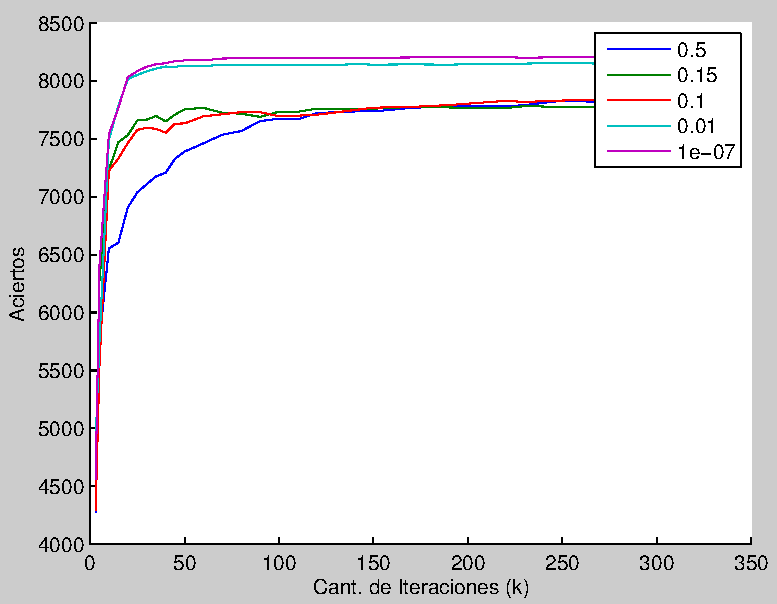
\includegraphics[scale=0.8]{imagenes/aciertos.pdf}
\end{center}
\caption{Gráfico de aciertos vs cantidad de iteraciones.}
\label{fig:aciertos-vs-k}
\end{figure}

En la figura (\ref{fig:tiempo-vs-k}), se muestra el tiempo de la ejecución del programa son contar el tiempo que tarda en
cargar la matriz de covarianza, para distintos valores de delta.

\begin{figure}[h]
\begin{center}
  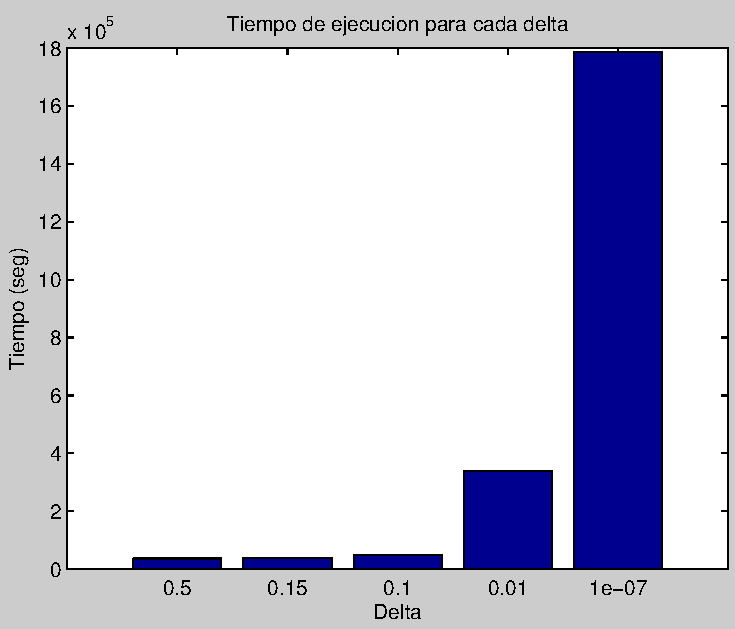
\includegraphics[scale=0.8]{imagenes/tiempos.pdf}
\end{center}
\caption{Gráfico de tiempo de ejecución vs delta.}
\label{fig:tiempo-vs-k}
\end{figure}
\vspace{0.5cm}

\clearpage

\section{Discusión}

Los resultados obtenidos corroboran que si se descartan demasiados componentes principales el método se vuelve ineficaz. Esto a la vez 
depende del valor de delta escogido. Cuanto mayor es delta, mas empeoran los resultados al quitar muchas componentes.

Al calcular los autovectores con mucha precisión se requieren pocas componentes para obtener los 
mismo resultados que utilizando menos precisión con muchas componentes. 
En concreto utilizando delta 0.1 se requieren como mínimo unas 200 componentes para el nivel óptimo de aciertos, mientras que con delta 0.01
se requieren solo 60.

Esto es una relación de compromiso teniendo en cuenta que cuanto menor es delta, se requiere mayor tiempo de ejecución.
Relación que se puede desempatar cuando se observa que según el delta hay valores máximos de aciertos , y que es mayor en cuanto el delta es menor.
Como se observa en el gráfico la diferencia entre los niveles de aciertos son importantes para los delta 0.1 y 0.01.

Luego para deltas menores a 0.01 el nivel de acierto no se ve incrementado considerablemente y teniendo en cuenta que si se incrementa el tiempo de
ejecución, significa que no tiene mucho sentido utilizar $deltas < 0.01$

\vspace{0.5cm}

\clearpage

\section{Conclusiones}
El problema del reconocimiento óptico de de dígitos fue resuelto satisfactoriamente ya que se encontraron métodos 
confiables, automatizables y precisos encontrado efectividad en el orden del 80\% para los 10000 casos de test utilizados.

Dentro de las técnicas utilizadas para encontrar los autovectores, se exploraron la resolución por medio de factorización QR y 
método de la potencia. Encontrando el primero altamente ineficiente para nuestra aplicación, clasificable como inutilizable en la practica.
Utilizando el método de la potencia encontramos resultados de precisión , con tiempos de ejecución aceptables.

Queda abierta la generalización del método al conjuntos de todos lo caracteres del español, en el cual es posible que se obtengan también 
buenos resultados.



\vspace{0.5cm}

\clearpage

\section{Apéndices}

\makeatletter
\def\PY@reset{\let\PY@it=\relax \let\PY@bf=\relax%
    \let\PY@ul=\relax \let\PY@tc=\relax%
    \let\PY@bc=\relax \let\PY@ff=\relax}
\def\PY@tok#1{\csname PY@tok@#1\endcsname}
\def\PY@toks#1+{\ifx\relax#1\empty\else%
    \PY@tok{#1}\expandafter\PY@toks\fi}
\def\PY@do#1{\PY@bc{\PY@tc{\PY@ul{%
    \PY@it{\PY@bf{\PY@ff{#1}}}}}}}
\def\PY#1#2{\PY@reset\PY@toks#1+\relax+\PY@do{#2}}

\expandafter\def\csname PY@tok@gd\endcsname{\def\PY@tc##1{\textcolor[rgb]{0.63,0.00,0.00}{##1}}}
\expandafter\def\csname PY@tok@gu\endcsname{\let\PY@bf=\textbf\def\PY@tc##1{\textcolor[rgb]{0.50,0.00,0.50}{##1}}}
\expandafter\def\csname PY@tok@gt\endcsname{\def\PY@tc##1{\textcolor[rgb]{0.00,0.25,0.82}{##1}}}
\expandafter\def\csname PY@tok@gs\endcsname{\let\PY@bf=\textbf}
\expandafter\def\csname PY@tok@gr\endcsname{\def\PY@tc##1{\textcolor[rgb]{1.00,0.00,0.00}{##1}}}
\expandafter\def\csname PY@tok@cm\endcsname{\let\PY@it=\textit\def\PY@tc##1{\textcolor[rgb]{0.25,0.50,0.50}{##1}}}
\expandafter\def\csname PY@tok@vg\endcsname{\def\PY@tc##1{\textcolor[rgb]{0.10,0.09,0.49}{##1}}}
\expandafter\def\csname PY@tok@m\endcsname{\def\PY@tc##1{\textcolor[rgb]{0.40,0.40,0.40}{##1}}}
\expandafter\def\csname PY@tok@mh\endcsname{\def\PY@tc##1{\textcolor[rgb]{0.40,0.40,0.40}{##1}}}
\expandafter\def\csname PY@tok@go\endcsname{\def\PY@tc##1{\textcolor[rgb]{0.50,0.50,0.50}{##1}}}
\expandafter\def\csname PY@tok@ge\endcsname{\let\PY@it=\textit}
\expandafter\def\csname PY@tok@vc\endcsname{\def\PY@tc##1{\textcolor[rgb]{0.10,0.09,0.49}{##1}}}
\expandafter\def\csname PY@tok@il\endcsname{\def\PY@tc##1{\textcolor[rgb]{0.40,0.40,0.40}{##1}}}
\expandafter\def\csname PY@tok@cs\endcsname{\let\PY@it=\textit\def\PY@tc##1{\textcolor[rgb]{0.25,0.50,0.50}{##1}}}
\expandafter\def\csname PY@tok@cp\endcsname{\def\PY@tc##1{\textcolor[rgb]{0.74,0.48,0.00}{##1}}}
\expandafter\def\csname PY@tok@gi\endcsname{\def\PY@tc##1{\textcolor[rgb]{0.00,0.63,0.00}{##1}}}
\expandafter\def\csname PY@tok@gh\endcsname{\let\PY@bf=\textbf\def\PY@tc##1{\textcolor[rgb]{0.00,0.00,0.50}{##1}}}
\expandafter\def\csname PY@tok@ni\endcsname{\let\PY@bf=\textbf\def\PY@tc##1{\textcolor[rgb]{0.60,0.60,0.60}{##1}}}
\expandafter\def\csname PY@tok@nl\endcsname{\def\PY@tc##1{\textcolor[rgb]{0.63,0.63,0.00}{##1}}}
\expandafter\def\csname PY@tok@nn\endcsname{\let\PY@bf=\textbf\def\PY@tc##1{\textcolor[rgb]{0.00,0.00,1.00}{##1}}}
\expandafter\def\csname PY@tok@no\endcsname{\def\PY@tc##1{\textcolor[rgb]{0.53,0.00,0.00}{##1}}}
\expandafter\def\csname PY@tok@na\endcsname{\def\PY@tc##1{\textcolor[rgb]{0.49,0.56,0.16}{##1}}}
\expandafter\def\csname PY@tok@nb\endcsname{\def\PY@tc##1{\textcolor[rgb]{0.00,0.50,0.00}{##1}}}
\expandafter\def\csname PY@tok@nc\endcsname{\let\PY@bf=\textbf\def\PY@tc##1{\textcolor[rgb]{0.00,0.00,1.00}{##1}}}
\expandafter\def\csname PY@tok@nd\endcsname{\def\PY@tc##1{\textcolor[rgb]{0.67,0.13,1.00}{##1}}}
\expandafter\def\csname PY@tok@ne\endcsname{\let\PY@bf=\textbf\def\PY@tc##1{\textcolor[rgb]{0.82,0.25,0.23}{##1}}}
\expandafter\def\csname PY@tok@nf\endcsname{\def\PY@tc##1{\textcolor[rgb]{0.00,0.00,1.00}{##1}}}
\expandafter\def\csname PY@tok@si\endcsname{\let\PY@bf=\textbf\def\PY@tc##1{\textcolor[rgb]{0.73,0.40,0.53}{##1}}}
\expandafter\def\csname PY@tok@s2\endcsname{\def\PY@tc##1{\textcolor[rgb]{0.73,0.13,0.13}{##1}}}
\expandafter\def\csname PY@tok@vi\endcsname{\def\PY@tc##1{\textcolor[rgb]{0.10,0.09,0.49}{##1}}}
\expandafter\def\csname PY@tok@nt\endcsname{\let\PY@bf=\textbf\def\PY@tc##1{\textcolor[rgb]{0.00,0.50,0.00}{##1}}}
\expandafter\def\csname PY@tok@nv\endcsname{\def\PY@tc##1{\textcolor[rgb]{0.10,0.09,0.49}{##1}}}
\expandafter\def\csname PY@tok@s1\endcsname{\def\PY@tc##1{\textcolor[rgb]{0.73,0.13,0.13}{##1}}}
\expandafter\def\csname PY@tok@sh\endcsname{\def\PY@tc##1{\textcolor[rgb]{0.73,0.13,0.13}{##1}}}
\expandafter\def\csname PY@tok@sc\endcsname{\def\PY@tc##1{\textcolor[rgb]{0.73,0.13,0.13}{##1}}}
\expandafter\def\csname PY@tok@sx\endcsname{\def\PY@tc##1{\textcolor[rgb]{0.00,0.50,0.00}{##1}}}
\expandafter\def\csname PY@tok@bp\endcsname{\def\PY@tc##1{\textcolor[rgb]{0.00,0.50,0.00}{##1}}}
\expandafter\def\csname PY@tok@c1\endcsname{\let\PY@it=\textit\def\PY@tc##1{\textcolor[rgb]{0.25,0.50,0.50}{##1}}}
\expandafter\def\csname PY@tok@kc\endcsname{\let\PY@bf=\textbf\def\PY@tc##1{\textcolor[rgb]{0.00,0.50,0.00}{##1}}}
\expandafter\def\csname PY@tok@c\endcsname{\let\PY@it=\textit\def\PY@tc##1{\textcolor[rgb]{0.25,0.50,0.50}{##1}}}
\expandafter\def\csname PY@tok@mf\endcsname{\def\PY@tc##1{\textcolor[rgb]{0.40,0.40,0.40}{##1}}}
\expandafter\def\csname PY@tok@err\endcsname{\def\PY@bc##1{\setlength{\fboxsep}{0pt}\fcolorbox[rgb]{1.00,0.00,0.00}{1,1,1}{\strut ##1}}}
\expandafter\def\csname PY@tok@kd\endcsname{\let\PY@bf=\textbf\def\PY@tc##1{\textcolor[rgb]{0.00,0.50,0.00}{##1}}}
\expandafter\def\csname PY@tok@ss\endcsname{\def\PY@tc##1{\textcolor[rgb]{0.10,0.09,0.49}{##1}}}
\expandafter\def\csname PY@tok@sr\endcsname{\def\PY@tc##1{\textcolor[rgb]{0.73,0.40,0.53}{##1}}}
\expandafter\def\csname PY@tok@mo\endcsname{\def\PY@tc##1{\textcolor[rgb]{0.40,0.40,0.40}{##1}}}
\expandafter\def\csname PY@tok@kn\endcsname{\let\PY@bf=\textbf\def\PY@tc##1{\textcolor[rgb]{0.00,0.50,0.00}{##1}}}
\expandafter\def\csname PY@tok@mi\endcsname{\def\PY@tc##1{\textcolor[rgb]{0.40,0.40,0.40}{##1}}}
\expandafter\def\csname PY@tok@gp\endcsname{\let\PY@bf=\textbf\def\PY@tc##1{\textcolor[rgb]{0.00,0.00,0.50}{##1}}}
\expandafter\def\csname PY@tok@o\endcsname{\def\PY@tc##1{\textcolor[rgb]{0.40,0.40,0.40}{##1}}}
\expandafter\def\csname PY@tok@kr\endcsname{\let\PY@bf=\textbf\def\PY@tc##1{\textcolor[rgb]{0.00,0.50,0.00}{##1}}}
\expandafter\def\csname PY@tok@s\endcsname{\def\PY@tc##1{\textcolor[rgb]{0.73,0.13,0.13}{##1}}}
\expandafter\def\csname PY@tok@kp\endcsname{\def\PY@tc##1{\textcolor[rgb]{0.00,0.50,0.00}{##1}}}
\expandafter\def\csname PY@tok@w\endcsname{\def\PY@tc##1{\textcolor[rgb]{0.73,0.73,0.73}{##1}}}
\expandafter\def\csname PY@tok@kt\endcsname{\def\PY@tc##1{\textcolor[rgb]{0.69,0.00,0.25}{##1}}}
\expandafter\def\csname PY@tok@ow\endcsname{\let\PY@bf=\textbf\def\PY@tc##1{\textcolor[rgb]{0.67,0.13,1.00}{##1}}}
\expandafter\def\csname PY@tok@sb\endcsname{\def\PY@tc##1{\textcolor[rgb]{0.73,0.13,0.13}{##1}}}
\expandafter\def\csname PY@tok@k\endcsname{\let\PY@bf=\textbf\def\PY@tc##1{\textcolor[rgb]{0.00,0.50,0.00}{##1}}}
\expandafter\def\csname PY@tok@se\endcsname{\let\PY@bf=\textbf\def\PY@tc##1{\textcolor[rgb]{0.73,0.40,0.13}{##1}}}
\expandafter\def\csname PY@tok@sd\endcsname{\let\PY@it=\textit\def\PY@tc##1{\textcolor[rgb]{0.73,0.13,0.13}{##1}}}

\def\PYZbs{\char`\\}
\def\PYZus{\char`\_}
\def\PYZob{\char`\{}
\def\PYZcb{\char`\}}
\def\PYZca{\char`\^}
\def\PYZam{\char`\&}
\def\PYZlt{\char`\<}
\def\PYZgt{\char`\>}
\def\PYZsh{\char`\#}
\def\PYZpc{\char`\%}
\def\PYZdl{\char`\$}
\def\PYZti{\char`\~}
% for compatibility with earlier versions
\def\PYZat{@}
\def\PYZlb{[}
\def\PYZrb{]}
\makeatother


\subsection{Apéndice A: Enunciado del TP}

\subsection{Apéndice B}

\subsection{Apéndice C}

% \subsubsection{MMMatrix.cpp}
% \input{secciones/codigo/MMMatrix.tex}

\vspace{0.5cm}

\clearpage

\section{Referencias}
% \begin{enumerate}
% 	\item Serie de Cosenos de Fourier - Wolfram MathWorld \\
% 	link: \emph{http://mathworld.wolfram.com/FourierCosineSeries.html} \\
% 	\item USC-SIPI Image Database - University of California, Signal and Image Processing Institute \\
% 	link: \emph{http://sipi.usc.edu/database/} \\
% 	\item Teorema Central del Limite - Blaiotta, Delieutraz (2004) \\
% 	link: \emph{http://www.itescam.edu.mx/principal/sylabus/fpdb/recursos/r75990.PDF} \\
% \end{enumerate}
\vspace{0.5cm}

\end{document}
